%%
%% Kapitel
%%
\chapter{Auswertung}
Im Folgenden werden die Ergebnisse aus den Experimenten des lezten Kapitels besprochen und m\"ogliche Verbesserungen angesprochen.

\section{Ergebnisse}
Bei \textbf{Sentiment Analysis} werden durch die Sprachmodelle schnell bessere Ergebnisse erreicht als ohne. Besonders die nicht-transformerbasierten Modelle sind zeitlich bei der Ausf\"uhrung sehr gut, die Genauigkeitswerte sind mit \"uber 80\% durchaus wettbewerbsf\"ahig (s. Abbildung \ref{fig:acc_sentiment}). Besonders \textbf{ULMFit} scheint gut geeignet f\"ur diese Aufgabe, da auch die Verarbeitungszeit hier, nicht wie bei den Transformer-Modellen, dem Datensatz angemessen ist. Ist ein gro{\ss}er Datensatz vorhanden, kann auch entsprechend gut trainiert werden. Die transformerbasierten Modelle scheinen deutlich resistenter gegen \textbf{Overfitting} auch bei kleinen Datens\"atzen zu sein, brauchen aber langes Training, um wirklich hohe Genauigkeiten zu erreichen. Das Problem scheint hierbei haupts\"achlich bei der Multi-Klassen Klassifizierung zu liegen, da diese Modelle l\"anger brauchen, um \"uber zwei Klassen hinaus zu klassifizieren. Die deutlich l\"angere Auf\"uhrungszeit stammt aus der h\"oheren Komplexit\"at der Transformer-Modelle.\\
\begin{figure}[!ht]
\centering
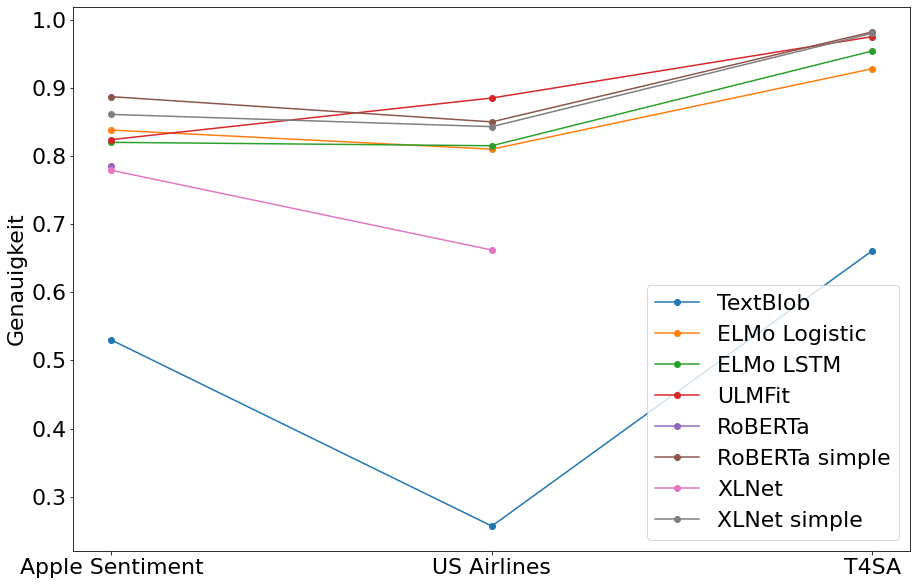
\includegraphics[height=8cm]{pics/accuracies_sentiment.png}
\caption{Genauigkeiten bei Sentiment Analysis}
\label{fig:acc_sentiment}
\end{figure}
Zur \textbf{Stance detection} scheinen LSTM-Modelle wie \textbf{ULMFit} weniger gut geeignet, hier werden die besten Ergebnisse durch Einsatz des \textbf{RoBERTa}-Modells mit \textbf{SimpleTransformers} erzielt, wie aus Abbildung \ref{fig:acc_stance} hervorgeht.
\begin{figure}[!ht]
\centering
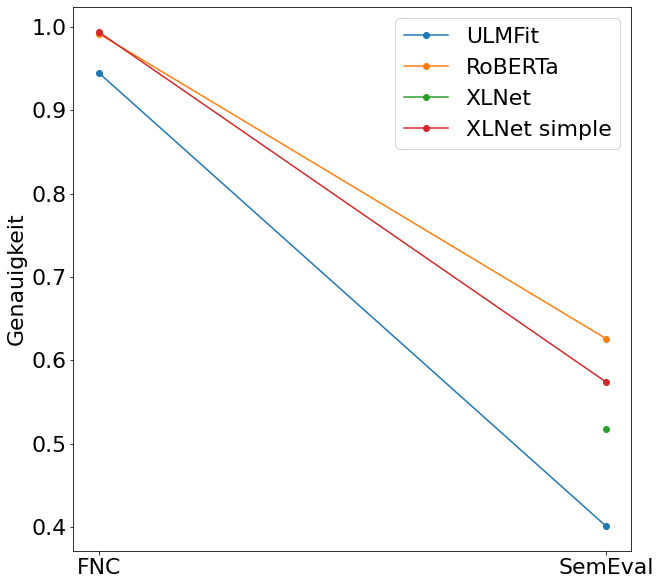
\includegraphics[height=8cm]{pics/accuracies_stance.png}
\caption{Genauigkeiten bei Stance Detection}
\label{fig:acc_stance}
\end{figure}
Aus den Graphen kann gefolgert werden, dass die mittels \textbf{SimpleTransformers} abgestimmten Modelle sehr effizient sind. Die Bibliothek ist offensichtlich gut anzuwenden und bringt sehr gute Ergebnisse. \\
Wie schon erw\"ahnt hat die Qualit\"at der und die Quantit\"at in den Datens\"atzen eine hohe Auswirkung auf das Ergebnis, dennoch kann gesagt werden, dass, wenn richtig konfiguriert, die urspr\"ungliche Transformer-Architektur der der XL-Transformer \"uberlegen ist.

\section{Ausblick}
In nachfolgenden Arbeiten kann die Trainingszeit und die Anzahl der getesteten Datensa\"atze erh\"oht werden, da die meisten Modelle von mehr Trainingszeit profitieren k\"onnen. Weiterhin k\"onnen auch bei der Textverarbeitung angebracht werden: Hierbei kann \textbf{Stemming} angewendet werden. Dadurch werden die W\"orter in ihre Grundform umgewandelt mit vorausgehenden oder nachfolgenden Silben als separate Tokens. Aus dem Wort "`playing"' werden so z.B. die zwei Tokens <play> und <ing>. Diese Art der \textbf{Tokenization} ist f\"ur den Einsatz mit Sprachmodellen am besten geeignet, da auch in diesen nicht alle Vokabeln einer Sprache enthalten sein k\"onnen - das w\"are schlicht ein zu gro{\ss}es Vokabular. Durch \textbf{Stemming} wird gew\"ahrleistet, dass die meisten W\"orter, sowie die jeweilige Pr\"afix und Suffix je einem Vektor zugeordnet werden k\"onnen (sollten keine Rechtschreibfehler enthalten sein).\\
Da \textbf{NLP} ein sehr weit verbreitetes Thema ist, werden auch in den n\"achsten Jahren immer weitere Sprachmodelle ver\"offentlicht werden, die in den unterschiedlichen Aufgabenstellungen St\"arken oder auch Schw\"achen haben werden und entsprechend getestet werden sollten.
